\documentclass[../main.tex]{subfiles}

\begin{document}

\chapter{Algorithm Complexity Analysis}
\label{chapter_algorithm_analysis}
When a software program runs on a machine, we  genuinely care about the \textit{hardware space} and the \textit{running time} that it takes to complete the execution of the program; space and running time is the cost we need to pay to get the problem solved. The lower the cost, the happier we would be. Thus, \texttt{space} and \texttt{running time} are two metrics we use to evaluate the performance of programs, or rather say, algorithms. 

Now, if I ask you the question, "How to evaluate the performance of algorithms?" Do not go low and tell me, "You just write the code and run it on a computer?" Because here is the reality: (a) These two metrics are mostly possible to vary as using different the physical machine and the programming languages, and (b) The cost will be too high. First, when we are solving a problem, we would always try to come up with many possible solutions--algorithms. Implementing and running all candidates just boost your cost of labor and finance. Second, even at the best case, you only have one candidate, but what if your designated machine can not load the program due to the memory limit, what if your algorithm takes millions of years to run, would you prefer to sit and wait? 

With these situation, it is obvious that we need  to \textit{predict} algorithm's performance--running time and space--without implementing or running on a particular machine, and meanwhile the prediction should be independent of the hardwares. In this chapter, we will study the complexity analysis method that strives to enable us such ability.  The space complexity is mostly obvious and way easier to obtain compared with its counterpart-time complexity. This decides that in this chapter, the analysis of time complexity will outweigh the pages we spent on space complexity. Before we dive into a plethora of algorithms and data structures, learning the complexity analysis techniques can help us evaluate each algorithm. 


% We organize the chapter:
% \begin{enumerate}
%     \item Introduction
%     \item Asymptotic notations
%     \item Amortized Analysis
%     \item Hands-on Examples
% \end{enumerate}

\section{Introduction}
In reality, it is impossible to predict the exact behavior of an algorithm, thus complexity analysis only try to extract the main influencing factors and ignore some trivial details. The complexity analysis is thus only \textit{approximate}, but it works. 

\paragraph{What are the main influencing factors? }

Imagine sorting an array of integers with size 10 and size 10,000,000. The time and space it takes to these two input size will mostly be a huge difference. Thus, the number of items in the \textit{input size} is a straightforward factor. Assume we use $n$ to denote the size of the input, and the complexity analysis will define an expression of the running time as $T(n)$ and the space as $S(n)$. 

In complexity analysis, RAM model is based upon, where instructions/operators are executed one after another, without concurrency. Therefore, the running time of algorithm on a particular input can be expressed as counting the number of \textit{operations or ``steps''} to run. 

\paragraph{What are the difference cases?}

Yet, when two input instance has exactly the same size, but with different values, such that one array where the input array is already sorted, and the other is totally random, the time it takes to these two cases will possibly vary, depending on the sorting algorithm that you chose. In complexity analysis, \textit{best-case}, \textit{worst-case}, \textit{average-case} complexity analysis is used to differentiate the behavior of the same algorithm applied on different input instance.  
\begin{enumerate}
    \item \textbf{Worst-case}: The behavior of the algorithm or an operation of a data structure with respect to the worst possible case of input instance.  This gave us a way to measure the upper bound on the running time for any input, which is denoted as $O$. Knowing it gives us a guarantee that the algorithm will never take any longer. 
    \item \textbf{Average-case}:  The expected behavior when the input is randomly drawn from a given distribution. Average case running time is used as an estimate complexity for a normal case. The expected case here offers us asymptotic bound $\Theta$.  Computation of average-case running time entails knowing all possible input sequences, the probability distribution of occurrence of these sequences, and the running times for the individual sequences. Often it is assumed that all inputs of a given size are equally likely. 
    \item \textbf{Best-case}: The possible best behavior when  the input data is arranged in a way, that your algorithms run least amount of time. Best case analysis can lead us to the lower bound $\Omega$ of an algorithm or data structure. 
\end{enumerate}

\paragraph{Toy Example: Selection Sort} Given a list of integers, sort the item incrementally.
\begin{lstlisting}[numbers=none]
For example, given the list A=[10, 3, 9, 2, 8, 7, 9], the sorted list will be:
A=[2, 3, 7, 8, 9, 9, 10].
\end{lstlisting}
There are many sorting algorithms, in this case, let us examine the \textit{selection sort}. Given the input array $A$, and size to be $n$, we have index $[0, n-1]$. In selection sort, each time we select the current largest item and swap it with item at its corresponding position in the sorted list, thus dividing the list into two parts: unsorted list on the left and sorted list on the right. For example, at the first pass, we choose 10 from $A[0,n-1]$ and swap it with $A[n-1]$, which is 9;  at the second pass, we choose the largest item 9 from $A[0,n-2]$ and swap it with 7 at $A[n-2]$, and so. Totally, after $n-1$ passes we will get an incrementally sorted array. More details of selection sort can be found in Chapter~\ref{chapter_sorting}. 

In the implementation, we use \texttt{ti} to denote the target position and \texttt{li} the index of the largest item which can only get by scanning. We show the Python code:
\begin{lstlisting}[language=Python]
def selectSort(a):                       cost           times
  '''Implement selection sort'''
  n = len(a)
  for i in range(n - 1): #n-1 passes, 
    ti = n - 1 -i                         c             n-1        
    li = 0                                c             n-1
    for j in range(n - i):
      if a[j] > a[li]:                    c \sum_{i=0}^{n-2}(n-i) 
        li = j                            c \sum_{i=0}^{n-2}(n-i)
    # swap li and ti
    print('swap', a[li], a[ti])
    a[ti], a[li] = a[li], a[ti]           c            n-1
    print(a)
  return a
\end{lstlisting}
First, we ignore the distinction between different operation types and treat all alike with a cost of $c$. In the above code, the line that comes with notations--\texttt{cost} and \texttt{times}--are operations. In line $5$, we first point at the target position \texttt{ti}. Because of the \texttt{for} loop above it, this operation will be called $n-1$ times. Same for line $6$ and $12$. For operation in line $8$ and $9$, the times it operated is denoted as $\sum_{i=0}^{n-2}(n-i)$ due to two nested \texttt{for} loops. And the range of $j$ is dependable of the outer loop with $i$.  We get our running time $T(n)$ by summing up these cost on the variable of $i$.
\begin{align}
\label{complexity_eq_1}
    T(n) &= 3c*(n-1) + \sum_{i=0}^{n-2} {2c(n-i)}\\
    &= 3c*(n-1) + 2c (n+(n-1)+(n-2)+...+2) \notag \\
    &= 3c*(n-1) + 2c (\frac{(n-1)*(2+n)}{2})\notag \\
    &=cn^2+cn-2+3cn-3c\notag \\
    &=cn^2+4cn-3c-2\label{complexity_eq_1_2} \\
    &=an^2+bn+c\label{complexity_eq_1_3}
\end{align}
We use three constants $a, b, c$ to rewrite Eq. \ref{complexity_eq_1_2} with Eq.\ref{complexity_eq_1_3}. 

In the case of sorting, an incrementally sorted array will potentially be the best-cases that takes the lest running time and on the other hand decrementally sorted array will be the worst-case. However, in the example of selection sorted array, even if the input is perfect sorted, the algorithm does not consider this case, it still runs n-1 passes, each pass it still scans from a fixed size of window to find the largest item (you would only know it is the largest by looking all cases). Thus, in this case, the best-case, worst-case, and average-case all happens to have the same running time shown in Eq.~\ref{complexity_eq_1_3}. 


%%%%%%%%%%%%%%%%%%%%%%%%%%%Asymptotic notations%%%%%%%%%%%%%%%%%%%%%%%%%%%%%%%%%
\section{Asymptotic Notations}
\paragraph{Order of Growth and Asymptotic Running Time} In Equation~\ref{complexity_eq_1_3} we end up with three constant a, b, c and two terms with order  $n^2$ and $n$. When the input is large enough, all the lower order terms, even if with large constant,  will become relatively insignificant to the highest term; we thus neglect the lower terms and end up with $an^2$. Further, we neglect the constant coefficient $a$ for the same reason. However, we can not say $T(n)=n^2$, because we know mathematically speaking, it is wrong. 
\begin{figure}[h!]
    \centering
    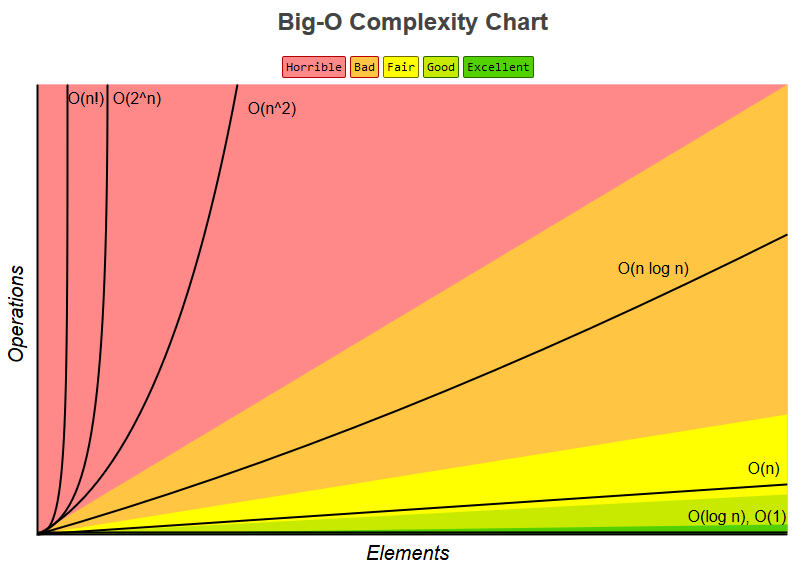
\includegraphics[width=0.8\columnwidth]{fig/big_o_complexity_chart.png}
    \caption{Order of Growth of Common Functions}
    \label{fig:big_o_complexity_chart}
\end{figure}

Instead, since we are only interested with property of $T(n)$ when $n$ is large enough, we say the relation between the original complexity function $an^2+bn+c$ is ``asymptotically equivalent to''  $n^2$, which reads ``$T(n)$ is is asymptotic to $n^2$'' and denoted as $T(n)=an^2+bn+c \asymp n^2$. Form Fig.~\ref{fig:big_o_complexity_chart}, we can visualize that when $n$ is large enough, the term $n$ is trivial compared with $n^2$. 

In this way, we manage to classify our complexity into a group of families, say, exponential $2^n$ or polynomial $n^2$.% For example, if the input size is $n$, then we can have functions like $f_1 = an+b$ and $f_2=an^2+bn+c$. But normally, we would only get the highest order of function, and simplified them to $g_1=n$ and $g_2=n^2$, with different notation. Function $f_1$ and $g_1$ are of the same order of magnitude or growth and $g_1$ can approach the curve of $f_1$ arbitrarily closely. The relation of them is  \textbf{asymptotic}, and denoted as $f_1 \asymp g_1$.

\subsubsection{Definition of Asymptotic Notations} We mentioned ``asymptotically equivalent'' relation, which can be formalized and  defined with $\Theta$-Notation as $T(n)=\Theta(n)$, one of the main three asymptotic notations--asymptotically equivalent, smaller, and larger--we will cover in this section.
\paragraph{$\Theta$-Notation}  For a given function $g(n)$, we define $\Theta(g(n))$(pronounced as ``big theta'') as a set of functions $\Theta(g(n))=\{f(n)\}$, that each $f(n)$ can be bounded by $g(n)$ by $0 \leq c_1g(n)\leq f(n)\leq c_2g(n)$ for all $n\geq n_0$ for positive constant $c_1$, $c_2$ and $n_0$. We show this relation in Fig.~\ref{fig:asym_notation}. Strictly speaking, we would write $f(n)\in\Theta(g(n))$ to indicate that $f(n)$ is just one member of the set of functions that $\Theta(g(n))$ can represent. However, in the field of computer science, we write  $f(n)=\Theta(g(n))$ instead. 

We say $g(n)$ is an  \textit{asymptotically tight bound} of $f(n)$.  For example, we can say $n^2$ is asymptotically tight bound for $2n^2+3n+4$ or $5n^2+3n+4$ or $3n^2$ or any other similar functions. We can denote our running time as $T(n)=\Theta(n^2)$.

\begin{figure}[!ht]
    \centering
    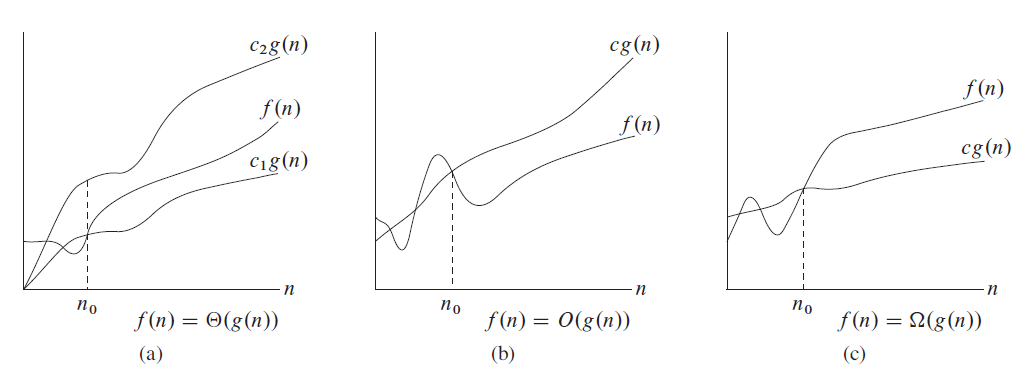
\includegraphics[width = 1\columnwidth]{fig/notations.png}
    \caption{Graphical examples for asymptotic notations. Replace f(n) with T(n) }
    \label{fig:asym_notation}
\end{figure}

\paragraph{$O$-Notation}  Further, we define the  \textit{asymptotically upper bound} of a set of functions $\{f(n)\}$ as $O(g(n))$(pronounced as ``big oh'' of $f(n)$), with $0 \leq  f(n)\leq cg(n)$ for all $n\geq n_0$ for positive constant $c$ and $n_0$. We show this relation in Fig.~\ref{fig:asym_notation}.

Note that $T(n) = \Theta(g(n))$ implies that $T(n)=O(g(n))$, but not the other way around. With $2n^2+3n+4$ or $5n^2+3n+4$ or $3n^2$, it also be denoted as $T(n)=O(n^2)$. Big Oh notation is widely applied in computer science to describe either the running time or the space complexity.

\paragraph{$\Omega$-Notation} It provides \textbf{asymptotic lower bound} running time. With $T(n)=\Omega(g(n))$(pronounced as ``big omega'') we represent a set of functions that $0 \leq cg(n) \leq f(n)$ for all $n\geq n_0$ for positive constant $c$ and $n_0$. 


\begin{bclogo}[couleur = blue!30, arrondi=0.1,logo=\bccrayon,ombre=true]{Does it mean that $O$ is worst-case, $\Theta$ is the average-case and $\Omega$ is the best-case? How does it relate to this three cases. }
\end{bclogo}

\subsubsection{Properties of Asymptotic Comparisons}
We should note that only if $f(n)=O(g(n))$ and $f(n)=\Omega(g(n))$, we can have $f(n)=\Theta(g(n))$.

\begin{table}[!ht]
\begin{small}
\centering
\noindent\captionof{table}{ Analog of Asymptotic Relation}
 \noindent \begin{tabular}{|p{0.4\columnwidth}|p{0.4\columnwidth}| }
  \hline
 Notation & Similar Relations   \\ \hline
$f(n)=\Theta(g(n))$  & $f(n)=g(n)$ \\\hline
$f(n)=O(g(n))$  &$f(n)\leq g(n)$\\ \hline
$f(n)=\Omega(g(n))$  & $f(n)\geq g(n)$\\\hline
\end{tabular}
  \label{tab:asymptotic_notation_property}
  \end{small}
\end{table}

It is fair to denote the relation of $g(n)$ and $f(n)$ to similar relation as between real numbers as shown in Table.~\ref{tab:asymptotic_notation_property}. Thus the properties of real numbers, such as transitivity, reflexivity, symmetry, transpose symmetry all holds for asymptotic notations. 

\section{Practical Guideline}
The previous two sections, we introduced the complexity function $T(n)$, how it is influenced by different cases of input instance--worst, average, and best cases, and how that we can use asymptotic notations to focus the complexity only on the dominant term in function $T(n)$. In this section, we would like to provide some practical guideline that arise in real application. 
\paragraph{Input Size and Running Time}
In general, the time taken by an algorithm grows with the size of the input, so it is universal to describe the running time of a program as a function of the size of its input. $f(n)$, with the input size denoted as $n$.

The notation of \textbf{input size} depends on specific problems and data structures. For example, the size of the array can be denoted as integer $n$, the total numbers of bits when it come to binary notation, and sometimes, if the input is matrix or graph, we need to use two integers such as $(m, n)$ for a two-dimensional matrix or $(V, E)$ for the vertices and edges in a graph. 

We use function $T$ to denote the running time. With input size of $n$, our running time can be denoted as $T(n)$. Given $(m, n)$, it can be $T(m, n)$. 

\paragraph{Worst-case Analysis is Preferred} 
In reality, worst-case input is chosen as our indicator over the best input and average input for: (a) best input is not representative; there is usually an input for the algorithm become trivial; (b) the average-input is sometimes very hard to define and measure; (3) In some cases, the worst-case input is very close to the average and to the observational input; (4)The algorithm with the best efficiency on the worst-case usually achieve the best performance. 

\paragraph{Relate Asymptotic Notations to Three Cases of Input Instance}
It might seemingly confusing about how the asymptotic notation relates to the three cases of input instance--worst-case, best-case, and average case. 

Think about it this way, asymptotic notations apply to any function that it abstract away some lower-term to characterize the property of the function when the input is large or infinite. Therefore, it has nothing to do with these three cases in this way. 

However, assume we are trying to characterize the complexity of an algorithm, and we analyzed its best-case and worst case input:
\begin{itemize}
    \item Worst-case: $T(n)=an^2+bn+c$, now we can say $T(n)=\Theta(n^2)$, which indicates that $T(n)=\Omega(n^2)$ and $T(n)=O(n^2)$.
    \item Best-case: $T(n)=an$, we can say $T(n)=\Theta(n)$, which indicates that $T(n)=\Omega(n)$ and $T(n)=O(n)$.
\end{itemize}
In order to describe the complexity of our algorithm in general; put aside the particular input instance. Such as the the average case analysis, which is typically hard to ``average'' between different input, we can  come up with an estimation, and safely say for the time complexity in general is $an\leq T(n)\leq an^2+bn+c$. This can be further expanded as:
\begin{equation}
    c_1n\leq an\leq T(n)\leq an^2+bn+c \leq c_2n^2
\end{equation}
Equivalently, we are safe to characterize a lower-bound based on best-case and an upper-bound based on the worst-case, thus we say the time complexity of our algorithm as $T(n)=\Omega(n), T(n)=O(n^2)$. 


\paragraph{Big Oh is a Popular Notation to Complexity Analysis}
As we have concluded that the worst-case analysis is both easy to get and good indicator of the overall complexity. Big Oh as the absolute upper bound of the worst-case would also indicate the upper bound of the algorithm in general. 

Even if we can get a tight bound for the algorithm as in the case of selection sort, it is always right to say that its an upper bound because $\Theta(g(n))$ is a subset of $O(g(n))$. This is like, we know dog is categorized as canine, and canine is in the type of mammal, thus, we are right to say that dog is a species of mammal. 




% \subsubsection{Four Types of Complexity Analysis}
%  As we will see in the remaining content of the book, different algorithm is affected differently with its input data distribution. We category this influence in three levels: worst-case, average-case, and best case.
% \begin{enumerate}
%     \item \textbf{Worst-case}: The behavior of the algorithm or an operation of a data structure with respect to the worst possible case of input instance.  This gave us a way to measure the upper bound on the running time for any input, which is denoted as $O$. Knowing it gives us a guarantee that the algorithm will never take any longer. 
%     \item \textbf{Average-case}:  The expected behavior when the input is randomly drawn from a given distribution. Average case running time is used as an estimate complexity for a normal case. The expected case here offers us asymptotic bound $\Theta$.  Computation of average-case running time entails knowing all possible input sequences, the probability distribution of occurrence of these sequences, and the running times for the individual sequences. Often it is assumed that all inputs of a given size are equally likely. 
%     \item \textbf{Best-case}: The possible best behavior when  the input data is arranged in a way, that your algorithms run least amount of time. Best case analysis can lead us to the lower bound $\Omega$ of an algorithm or data structure. 
% \end{enumerate}
% The selection algorithm's complexity will not be affected by its input, because no matter what data distribution is, we need to traverse the fixed range of array to find the largest item. For these type of algorithms, usually we have $T(n)=O(g(n))=\Theta(g(n))=\Omega(g(n))$. However, there are a lot of other algorithms that differs from different inputs. 

% All of these notations are applied to functions.  However, in the practical interviews, when the interviewer asks you to give the time and space complexity, you do not necessarily to give them the answer for each notation, you can just use $O$ to denote, with regarding to different cases introduced in the next section.  Here, we provide the most likely used growth rate plotted in Fig.~\ref{fig:big_o_complexity_chart}.


\section{Time Recurrence Relation}
We have studied recurrence relation throughly in Chapter.~\ref{chapter_recurrence_relation}. How does it relate to complexity analysis? We can represent either recursive function or iterative function with time recurrence relation. Therefore, the complexity analysis can be done in two steps: (1) get the recurrence relation and (2) solve the recurrence relation.
\begin{itemize}
    \item For recursive function, this representation is natural. For example, in the merge sort, it can be easily represented as $T(n)=2T(n/2)+O(n)$, that each step it divides a problem of size $n$ into two subproblems each with half size, and the cost to combine the solution of these two subproblems will be at most $n$, that is why we add $O(n)$.
    \item A time recurrence relation can be easily applied on iterative program too. Say, in the simple task where we try to search a target in a list array, we can write a recurrence relation function to it as $T(n)=T(n-1)+1$. Because, in the scanning process, one move reduce the problem to a smaller size, and the case of it is 1. Using the asymptotic notation, we can further write it as $T(n)=T(n-1)+O(1)$. Solving this recurrence relation straightforwardly through iteration method, we can have $T(n)=O(n)$. 
\end{itemize}

As in the chapter.~\ref{chapter_divide_and_conquer}, there are generally two ways of reducing a problem: divide and conquer and Reduce by Constant size, which is actually a non-homogenous recurrence relation. 

 In Chapter.~\ref{chapter_recurrence_relation}, we showed how to solve linear recurrence relation and get absolute answer, it was seemingly complex and terrifying. Good news, as complexity analysis is about estimating the cost, so we can loose ourselves a bit and sometimes a lower/upper bound is good enough, and the base case will almost always be $O(1)=1$. 
 
 \subsection{General Methods to Solve Recurrence Relation}
 We have shown in Chapter.~\ref{chapter_recurrence_relation} there are iterative method and mathematical induction as general methods to try to solve an easy recurrence relation. We demonstrate how these two methods can be used in solving time recurrence relations first. Additionally, we introduce recursion tree method. 
 \subsubsection{Iterative Method}
The most straightforward method for solving recurrence relation no matter its linear or non-linear is the \textit{iterative method}. Iterative method is a technique or procedure in computational mathematics that it iteratively replace/substitute each $a_n$ with its recurrence relation $\Psi(n, a_{n-1}, a_{n-2}, ..., a_{n-k})$ till all items ``disappear'' other than the initial values. Iterative method is also called substitution method. 

We demonstrate iteration with a simple non-overlapping recursion. 
\begin{align}
\label{complexity_eq_binary_search}
    T(n)&=T(n/2)+O(1)\\
    &=T(n/2^2)+O(1)+O(1)\notag\\
    &=T(n/2^3)+3O(1)\notag\\
    &=...\notag\\
    &=T(1)+kO(1)
\end{align}
We have $\frac{n}{2^k}=1$, we solve this equation and will get $k=\log_2 n$. Most likely $T(1)=O(1)$ will be the initial condition, we replace this, and we get $T(n)=O(\log_2 n)$.

However, when we try to apply iteration on the third recursion:  $T(n)=3T(n/4)+O(n)$. It might be tempting to assume that $T(n)=O(n\log n)$ due to the fact that $T(n)=2T(n/2)+O(n)$ leads to this time complexity.
\begin{align}
\label{complexity_non_overlap_1}
    T(n)&=3T(n/4)+O(n)\\
    &=3(3T(n/4^2)+n/4)+n=3^2T(n/4^2)+n(1+3/4)\notag\\
    &=3^2(3T(n/4^3)+n/4^2)+n(1+3/4)=3^3T(n/4^3)+n(1+3/4+3/4^2)\\
    &=...\\
    &=3^kT(n/4^k)+n\sum_{i=0}^{k-1}(\frac{3}{4})^{i}
\end{align}
\subsubsection{Recursion Tree}
Since the term of T(n) grows, the iteration can look messy. We can use recursion tree to better visualize the process of iteration. In a recursive tree, each node represents the value of a single subproblem, and a leaf would be a subproblem. As a start, we expand $T(n)$ as a node with value $n$ as root, and it would have three children each represents a subproblem $T(n/4)$. We further do the same with each leaf node, until the subproblem is trivial and be a base case. In practice, we just need to draw a few layers to find the rule. The cost will be the sum of costs of all layers.  The process can be seen in  Fig.~\ref{fig:recursive_tree}. 
\begin{figure}[!ht]
    \centering
    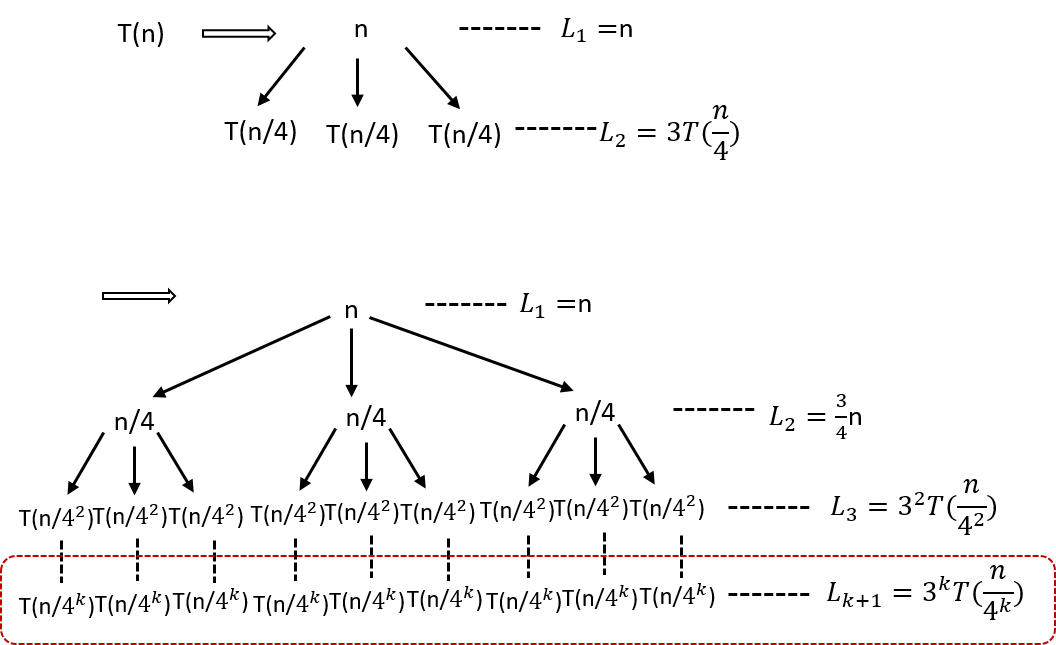
\includegraphics[width=0.98\columnwidth]{fig/recursion_tree_non_overlap.png}
    \caption{The process to construct a recursive tree for $T(n) = 3T(\floor*{n/4}) + O(n)$. There are totally k+1 levels. Use a better figure.  }
    \label{fig:recursive_tree}
\end{figure}
 In this case, it is the base case $T(1)$. Through the expansion with iteration and recursion tree, our time complexity function becomes:
\begin{align}
\label{complexity_non_overlap_2}
    T(n)&=\sum_{i=1}^{k}L_i + L_{k+1}\\
    &=n\sum_{i=1}^{k}(3/4)^{i-1}+3^kT(n/4^k)
\end{align}

In the process, we can see that Eq.~\ref{complexity_non_overlap_2} and Eq.~\ref{complexity_non_overlap_1} are the same.  Because $T(n/4^k)=T(1)=1$, we have $k=\log_4 n$. 
\begin{align}
\label{complexity_non_overlap_2}
    T(n)&\leq n\sum_{i=1}^{\infty}(3/4)^{k-1}+3^kT(n/4^k)\\
    &\leq 1/(1-3/4)n+3^{\log_4 n} T(1)= 4n+n^{log_4 3}
    &\leq 5n \\
    &=O(n)
\end{align}



\subsubsection{Mathematical Induction}
Mathematical induction is a mathematical proof technique, and is essentially used to prove that a property $P(n)$ holds for every natural number $n$, i.e. for $n=0, 1, 2, 3$, and so on. Therefore, in order to use induction, we need to make a \textit{guess} of the closed-form solution for $a_n$. Induction requires two cases to be proved. 
\begin{enumerate}
    \item 
 \textit{Base case:} proves that the property holds for the number $0$. 
\item \textit{Induction step:} proves that, if the property holds for one natural number $n$, then it holds for the next natural number $n+1$.
\end{enumerate}

For $T(n)=2\times T(n-1) +1, T_0 = 0$, we can have the following result by expanding $T(i), i \in [0, 7]$.
\begin{lstlisting}[numbers=none]
n    0 1 2 3 4 5 6 7
T_n  0 3 7 15 31 63 127
\end{lstlisting}
It is not hard that we find the rule and guess $T(n) = 2^n-1$. Now, we prove this equation by induction:
\begin{enumerate}
    \item Show that the basis is true: $T(0) = 2^0 -1 = 0$.
    \item Assume it holds true for $T(n-1)$. By induction, we get
    \begin{align}
        T(n)&=2T(n-1) + 1 \\
        &=2 (2^{n-1} - 1) + 1 \\
        &= 2^n -1
    \end{align}
    Now we show that the induction step holds true too. 
\end{enumerate}

\begin{bclogo}[couleur = blue!30, arrondi=0.1,logo=\bccrayon,ombre=true]{Solve $T(n)=T(n/2)+O(1)$ and $T(2n)\leq2T(n)+2n-1, T(2)=1$.}
\end{bclogo}
 
 \subsection{Solve Divide-and-Conquer Recurrence Relations}
All the previous recurrence relation, either homogeneous or non-homogeneous, they fall into the bucket of \textit{decrease and conquer} (maybe not right), and either is yet another type of recursion--Divide and Conquer. Same here, we ignore how we get such recurrence but focus on how to solve it. 

We write our divide and conquer recurrence relation using the time complexity function, there are two types as shown in Eq.\ref{divide_conquer_eq1}(n are divided equally) and E1.\ref{divide_conquer_eq2}(n are divided unequally):
\begin{equation}
    T(n)=aT(n/b)+f(n)
    \label{divide_conquer_eq1}
\end{equation}
where $a\leq 1, b>1$, and $f(n)$ is a given function, which usually has $f(n)= cn^k$.
\begin{equation}
    T(n)=\sum_{i=1}^{k}a_iT(n/b_i)+f(n)
    \label{divide_conquer_eq2}
\end{equation}
Considering that the first type is much more commonly seen that the other, we only learn how to solve the first type; in fact, at least, I assume you that within this book, the second type will never appear. 

\paragraph{Sit and Deduct} For simplicity, we assume $n=b^m$, so that $n/b$ is always integer. First, let us use the iterative method, and expand Eq.~\ref{divide_conquer_eq1} up till $n/b^m$ times so that $T(n)$ become $T(1)$:
\begin{align}
    T(n)&=aT(n/b)+cn^k\\
    &=a(aT(n/b^2)+c(n/b)^k)+cn^k\\
    &=a(a(T(n/b^3)+c(n/b^2)^k)+c(n/b)^k)+cn^k\\
    &\vdots\\
    &=a(a(\ldots T(n/b^m)+c(n/b^{m-1})^{k})+\ldots)+cn^k\\ 
    &=a(a(\ldots T(1)+cb^{k})+\ldots)+cn^k
\end{align}
Now, assume $T(1)=c$ for simplicity and for getting rid of this constant part in our sequence. Then,
\begin{equation}
    T(n)=ca^m+ca^{m-1}b^k+ca^{m-2}b^{2k}+\ldots+cb^{mk},
\end{equation}
which implies that
\begin{align}
T(n)&=c\sum_{i=0}^ma^{m-i}b^{ik}\\
&=ca^m\sum_{i=0}^m(\frac{b^k}{a})^i
\end{align}
So far, we get a geometric series, which is a good sign to get the closed-form expression. We first summarize all possible substitutions that will help our further analysis.
\begin{align}
    f(n)&=cn^k\\
    n&=b^m\\
    & \xrightarrow{} \\
    \label{eq_divide_conquer_sub_2}
    m&=\log_b n\\
    f(n)&=cb^{mk}\\
    a^m&=a^{\log_b n}=n^{\log_b a}\label{eq_divide_conquer_sub_1}
\end{align}
Depending on the relation between $a$ and $b^k$, there are three cases:
\begin{enumerate}
    \item $b^k < a$: In this case, $\frac{b^k}{a}<1$, so the geometric series converges to a constant even if $m$ goes to infinity. Then, we have an upper bound for $T(n)$, $T(n)<ca^m$, which converts to $T(n)=O(a^m)$. According to Eq.~\ref{eq_divide_conquer_sub_1}, we further get:
    \begin{equation}
        T(n)=O(n^{\log_b a})
    \end{equation}
    \item $b^k = a$: With $\frac{b^k}{a}=1$, $T(n)=O(a^mm)$. With Eq.~\ref{eq_divide_conquer_sub_1} and Eq.~\ref{eq_divide_conquer_sub_2}, our upper bound is:
    \begin{equation}
        T(n)=O(n^{\log_b a}\log_b n)
    \end{equation}
    \item $b^k > a$: In this case, we denote $\frac{b^k}{a}=d$ ($d$ is a constant and $d>1$). Use the standard formula for summing over a geometric series:
    \begin{align}
        T(n)&=ca^m\frac{d^{m+1}-1}{d-1}=O(a^m\frac{d^{m+1}-1}{d-1})\\
        &=O(b^{mk})=O(n^k)=O(f(n))
    \end{align}
\end{enumerate}



\subsubsection{Master Method} Comparison between $b^k$ and $a$ equals to the comparison between $b^{km}$ between $a^m$ . From the above substitution, it further equals to compare  $f(n)$ to $n^{\log_b a}$. This is when master method kicks in and we will see how it helps us to apply these three cases into real situation. 

Compare   $f(n)/c=n^k$ with  $n^{\log_b a}$. Intuitively, the larger of the two functions would dominate the solution to the recurrence. Now, we rephrase the three cases using the master method for the easiness of memorization.  
\begin{enumerate}
    \item If $n^k<n^{\log_b a}$, or say \textit{polynomially smaller} than by a factor of $n^{\epsilon}$ for some constant $\epsilon > 0$, we have:
     \begin{equation}
        T(n)=O(n^{\log_b a})
    \end{equation}
    \item If $n^k>n^{\log_b a}$, similarily, we need it to be polynomially larger than a factor of $n^{\epsilon}$ for some constant $\epsilon > 0$, we have:
         \begin{equation}
        T(n)=O(f(n))
    \end{equation}
    \item If $n^k=n^{\log_b a}$, then:
        \begin{equation}
        T(n)=O(n^{\log_b a}\log_b n)
    \end{equation}
   
\end{enumerate}

 


%%%%%%%%%%%%%%%%%%%%%%%%%%%%%%%%%%%%%%%%%%%%%%%%%%%%%%%%%%%%%%%%%%%%%%%%%%%%%%%%%%%%%
%%%%%%%%%%%%% Complexity Analysis
%%%%%%%%%%%%%%%%%%%%%%%%%%%%%%%%%%%%%%%%%%%%%%%%%%%%%%%%%%%%%%%%%%%%%%%%%%%%%%%%%%%%%%%%%
\subsection{Hands-on Example: Insertion Sort}
\label{sec_time_complexity}
In this section, we are expecting to see example that has different asymptotic bound as the input differs; where we focus more on the worst-case and average-case analysis. Along the analysis of complexity, we will also see how asymptotic notation can be used in equations or inequalities to assist the process. 

Because most of the time, the average-case running time will be asmptotically equal to the worst-case, thus we do not really try to analyze it at the first place. In the case of best-case, it would only matter if you know your application context fits right in, otherwise, it will be trivial and non-helpful in the comparison of multiple  algorithms. We will see example below. 

\paragraph{Insertion Sort: Worst-case and Best-case} There is another sorting algorithm--insertion sort--it sets aside another array $S$ to save the sorted items. At first, we can put the first item in which itself is already sorted. At the second pass, we put A[1] into the right position in $S$. Until the last item is handled, we return the sorted list. The code is:
\begin{lstlisting}[language=Python]
def insertionSort(a):
  '''implement insertion sort'''
  if not a or len(a) == 1:
    return a
  n = len(a)
  sl = [a[0]] + [None] *(n-1) # sorted list
  for i in range(1, n): # items to be inserted into the sorted
    key = a[i]
    j = i-1 

    while j >= 0 and sl[j] > key: # compare key from the last sorted element
      sl[j+1] = sl[j] # shift a[j] backward
      j -= 1
    sl[j+1] = key
    print(sl)
  return sl
\end{lstlisting}
For the first \texttt{for} loop in line 7, it will sure has $n-1$ passes. However, for the inner \texttt{while} loop, the real times of execution of statement in line 12 and 13 depends on the state between \texttt{sl} and \texttt{key}. If we try to sort the input array \texttt{a} incrementally such that A=[2, 3, 7, 8, 9, 9, 10], and if the input array is already sorted, then there will be no items in the sorted list can be larger than our key which result only the execution of line 14. This is the best case, we can denote the running time of the \texttt{while} loop by $\Omega(1)$ because it has constant running time at its best case. However, if the input array is a reversed as the desired sorting, which means it is decreasing sorted such as A=[10, 9, 9, 9, 7, 3, 2], then the inner \texttt{while} loop will has $n-i$, we denote it by $O(n)$. We can denote our running time equation as:
\begin{align}
    T(n)&=T(n-1)+O(n)\\
    &=O(n^2) \notag
\end{align}
And, 
\begin{align}
    T(n)&=T(n-1)+\Omega(1)\\
    &=\Omega(n)\notag
\end{align}
Using simple iteration, we can solve the math formula and have the asymptotic upper bound and lower bound for the time complexity of insertion sort. 

For the average case, we can assume that each time, we need half time of comparison of $n-i$, we can have the following equation:
\begin{align}
    T(n)&=T(n-1)+\Theta(n/2)\\
    &=T(n-2)+\Theta(\frac{n}{2}+\frac{n-1}{2}) \notag\\
    &=\Theta(n^2)\notag
\end{align}
For algorithm that is stable in complexity, we conventionally analyze its average performance, and it is better to use $\Theta$-notation in the running time equation and give the asymptotic tight bound like in the selection sort. For algorithm such as insertion sort, whose complexity varies as the input data distribution we conventionally analyze its worst-case and use $O$-notation.



% \paragraph{Simple example} These are just straightforward for us to analyze the running time. Sometimes, things become more obscure. Then, we need more advanced techniques to help us handle. For example, we use recurrence function to represent the the time we need when the problem decrease the size. Such that for one for loop, we can use $T(n)=T(n-1)+O(1)$, and for two nested for loops, normally $T(n)=T(n-1)+O(n)$ is enough to represent this situation. For a divide and conquer problem, we might get a recurrence function as $T(n) = T(n/2)+O(1)$. With recurrence function, the time complexity analysis is conveniently converted to a math problem and things get to be more interesting. We can divide the recurrence function into two types: non-overlapping as $T(n) = T(a*n/b)+f(n)$, and with over-lapping as $T(n) = T(a*n/b)+f(n)$. 


%%%%%%%%%%%%%%%%%%Amortiled analysis%%%%%%%%%%%%%
\section{*Amortized Analysis}
\label{sec_amortized_analysis}
There are two different ways to evaluate an algorithm/data structure: 

\begin{enumerate}
    \item Consider each operation separately: one that look each operation incurred in the algorithm/data structure separately and offers worst-case running time $O$ and average running time $\Theta$ for each operation. For the whole algorithm, it sums up on these two cases by how many times each operation is incurred.
    \item Amortized among a sequence of (related) operations: Amortized analysis can be used to show that the average cost of an operation is small, if one averages over a sequence of operations, even though a simple operation might be expensive. Amortized analysis guarantees the average performance of each operation in the worst case. 
\end{enumerate}

Amortized analysis does not purely look each operation on a given data structure separately, it averages time required to perform a sequence of different data structure operations over all performed operations. With amortized analysis, we might see that even though one single operation might be expensive, the amortized cost of this operation on all operations is small. Different from average-case analysis, probability will not be applied. From the example later we will see that amortized analysis view the data structure in applicable scenario, to complete this tasks, what is the average cost of each operation, and it is acheviable given any input. Therefore, the same time complexity, say $O(f(n))$, worst-case > amortized > average.

There are three types of amortized analysis:
\begin{enumerate}
    \item Aggregate Analysis:
    \item Accounting Method:
    \item Potential method: 
\end{enumerate}
%%%%%%%%%%%%%%%%%%space complexity%%%%%%%%%%%%%%%
\section{Space Complexity}
The analysis of space complexity is more straightforward, given that we are essentially the one who allocate space for the application. We simply link it to the size of items in the data structures. The only obscure is with \textit{recursive program} which takes space from stack but is hidden from the users by the programming language compiler or interpreter. The recursive program can be represented as a recursive tree, the maximums stack space it needs is decided by the height of the recursive tree, thus $O(h)$, given $h$ as the height.

\paragraph{Space and Time Trade-off} In the field of algorithm design, we can usually trade space for time efficiency or trade time for space efficiency. For example, if you put your algorithm on a backend server, we need to response the request of users, then decrease the response time if especially useful here. Normally we want to decrease the time complexity by sacrificing more space if the extra space is not a problem for the physical machine. But in some cases, decrease the time complexity is more important and needed, thus we need might go for alternative algorithms that uses less space but might with more time complexity. 

\section{Summary}
For your convenience, we provide a table that shows the frequent used recurrence equations' time complexity. 
\begin{figure}[h]
    \centering
    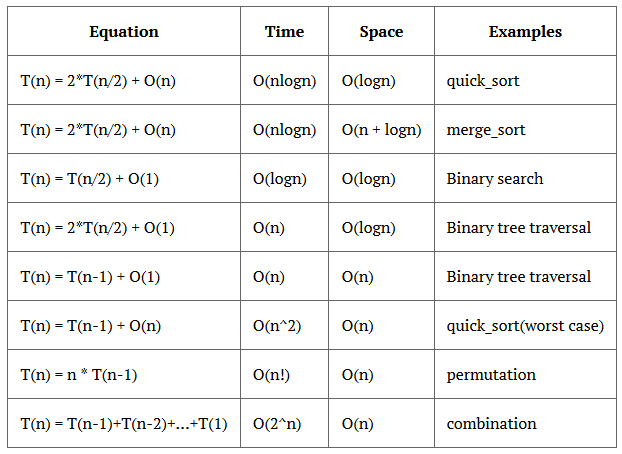
\includegraphics[width=1\columnwidth] {fig/complexity_cheatsheet.png}
    \caption{The cheat sheet for time and space complexity with recurrence function. If T(n) = T(n-1)+T(n-2)+...+T(1)+O(n-1) = $3^n$. They are called factorial, exponential, quadratic, linearithmic, linear, logarithmic, constant. }
    \label{fig:cheat_sheet}
\end{figure}

%%%%%%%%%%%%%%%%%%%%%%%%%Examples%%%%%%%%%%%%%%%%%%%%%%%%%
% \subsection{More Examples}
% \begin{examples}[resume]
% \item \textbf{ Pow(x, n) (50).}
    
%     Solution: T(n)= T(n/2)+O(1), the complexity is the same as the binary search, $O(logn)$.
% \begin{lstlisting}[language=Python]
% def myPow(self, x, n):
%     """
%     :type x: float
%     :type n: int
%     :rtype: float
%     """
%     if n==0:
%         return 1
%     if n<0:
%         n=-n
%         x=1.0/x
%     def helper(n):
%         if n==1:
%             return x
        
%         h = n//2
%         r = n-h
%         value = helper(h) #T(n/2), then we have O(1)
%         if r==h:                
%             return value*value
%         else: #r is going to be 1 bigger
%             return value*value*x
%     return helper(n)
% \end{lstlisting}
% \end{examples}


%%%%%%%%%%%%%%Cheat sheet%%%%%%%%%%%%%%%%%%%%%%
% \subsection{Big-O Cheat Sheet}
% \label{complexity_subsec_cheat_sheet}
% In this section, we provide the plotting of common seen time complexity functions (shown in Fig~\ref{fig:big_o_complexity_chart}): including $log_2{n}$, $n$, $n\log_2{n}$, $n^2$, $2^n$, and $n!$, so that we can sense the complexity change as the input size n increase. Resource found on \url{http://bigocheatsheet.com/}.


% \begin{table}[h]
% \begin{small}
% \centering
% \noindent\captionof{table}{ Explanation of Common Growth Rate}
%  \noindent \begin{tabular}{|p{0.15\columnwidth}|p{0.2\columnwidth}| p{0.65\columnwidth}|}
%   \hline
%  Growth Rate & Name & Example operations   \\ \hline
% $O(1)$  & Constant& append, get item, set item \\\hline
% $O(\log{n})$  &Logarithmic& binary search in the sorted array\\ \hline
% $O(n)$  & Liner & Copy, iteration\\ \hline
% $O(n\log{n})$  & Linear-Logarithmic& MergeSort, QuickSort\\ \hline
% $O(n^2)$  & Quadratic& Nested Loops\\ \hline
% $O(n^3)$  &Cubic& Matrix Multiplication\\ \hline
% $O(2^n)$  & Exponential& Backtracking, Combination\\ \hline
% $O(n!)$  & factorial & Permutation\\ \hline
% \end{tabular}
%   \label{tab:single_sequence}
%   \end{small}
% \end{table}

% Also, we provide the average and worst time and space complexity for the some classical data structure's operations (shown in Fig.~\ref{fig:data_structure_complexity}) and of algorithms (shown in Fig.~\ref{fig:data_structure_complexity}).
% \begin{figure}[h!]
%     \centering
%     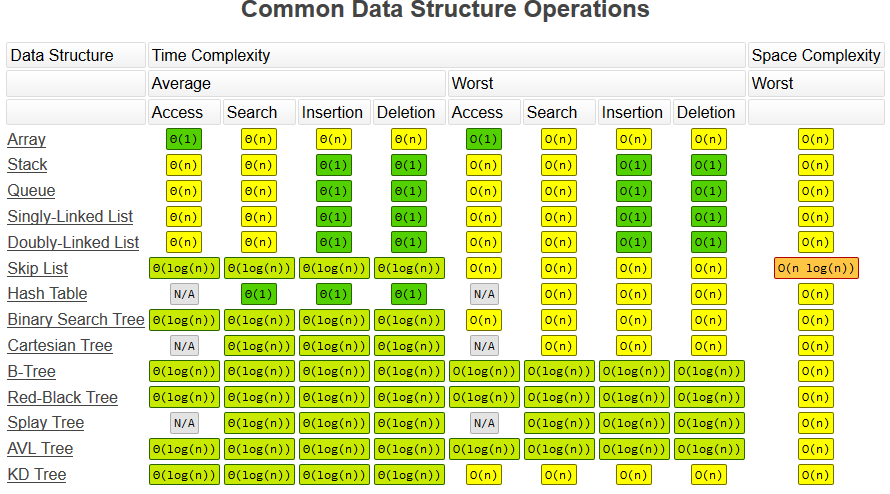
\includegraphics[width=0.9\columnwidth]{fig/common_data_structure_operations.png}
%     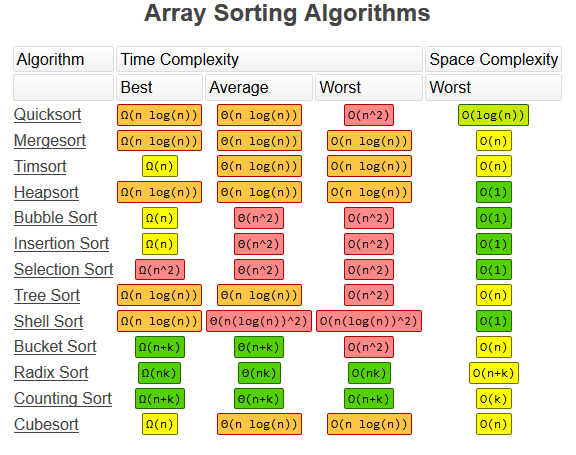
\includegraphics[width=0.9\columnwidth]{fig/array_sorting_algorithms.png}
%     \caption{Complexity of Common Data structures}
%     \label{fig:data_structure_complexity}
% \end{figure}

%%%%%%%%%%%%%%%%%%%%%%Exercise
\section{Exercises}
\subsection{Knowledge Check}
\begin{enumerate}
    \item Use iteration and recursion tree to get the time complexity of $T(n)=T(n/3)+2T(2n/3)+O(n)$. 
    \item Get the time complexity of $T(n)=2T(n/2)+O(n^2)$.
    \item $T(n)=T(n-1)+T(n-2)+T(n-3)+...+T(1)+O(1)$. 
\end{enumerate}
\end{document}